\documentclass[conference]{IEEEtran}
\IEEEoverridecommandlockouts
% The preceding line is only needed to identify funding in the first footnote. If that is unneeded, please comment it out.
\usepackage{cite}
\usepackage{rotating}
\usepackage{amsmath,amssymb,amsfonts}
% \usepackage[2107828]{easymcm}  % 载入 EasyMCM 模板文件
\usepackage{algorithmic}
\usepackage{graphicx}
\usepackage{booktabs}
\usepackage{textcomp}
\usepackage{xcolor}
% \def\BibTeX{{\rm B\kern-.05em{\sc i\kern-.025em b}\kern-.08em
%     T\kern-.1667em\lower.7ex\hbox{E}\kern-.125emX}}
\begin{document}

\title{A Model to Examine Evolutionary and Revolutionary Trends of Artists and Genres\\
{\footnotesize \textsuperscript{*}\iffalse Note: Sub-titles are not captured in Xplore and
should not be used \fi}
\thanks{\iffalse Identify applicable funding agency here. If none, delete this.\fi}
}

\author{\IEEEauthorblockN{\iffalse 1\textsuperscript{st} \fi Lizhang Chen}
\IEEEauthorblockA{\textit{School of Science} \\
\textit{Beijing Jiaotong University}\\
Beijing, China \\
lzchen@bjtu.edu.cn}

\iffalse
\and
\IEEEauthorblockN{2\textsuperscript{nd} Given Name Surname}
\IEEEauthorblockA{\textit{dept. name of organization (of Aff.)} \\
\textit{name of organization (of Aff.)}\\
City, Country \\
email address or ORCID}
\and
\IEEEauthorblockN{3\textsuperscript{rd} Given Name Surname}
\IEEEauthorblockA{\textit{dept. name of organization (of Aff.)} \\
\textit{name of organization (of Aff.)}\\
City, Country \\
email address or ORCID}
\and
\IEEEauthorblockN{4\textsuperscript{th} Given Name Surname}
\IEEEauthorblockA{\textit{dept. name of organization (of Aff.)} \\
\textit{name of organization (of Aff.)}\\
City, Country \\
email address or ORCID}
\and
\IEEEauthorblockN{5\textsuperscript{th} Given Name Surname}
\IEEEauthorblockA{\textit{dept. name of organization (of Aff.)} \\
\textit{name of organization (of Aff.)}\\
City, Country \\
email address or ORCID}
\and
\IEEEauthorblockN{6\textsuperscript{th} Given Name Surname}
\IEEEauthorblockA{\textit{dept. name of organization (of Aff.)} \\
\textit{name of organization (of Aff.)}\\
City, Country \\
email address or ORCID}\fi
}


\maketitle
\begin{abstract}
As part of an effort to understand the role music has played in collective human experience, 
we develop a method to quantify musical evolution. Our goal is to understand and measure the influence of 
previously produced music on new music and musical artists. Some artists can list a dozen or more other artists 
who they say influenced their own musical work. It has also been suggested that influence can be measured by the 
degree of similarity between song characteristics. This can be due to a sequence of small changes, a cooperative effort of artists, 
a series of influential artists, or a shift within society. \\ Many songs have similar sounds, and many artists have contributed to major 
shifts in the musical genre. By considering networks of songs and their musical characteristics, we can begin to capture the influence that musical 
artists have on each other. And, perhaps, we can also gain a better understanding of how music evolves through society over time. The influence network 
is established and analyzed deeply, and the influence index is established based on the centrality of network nodes: we establish the directed influence 
network among artists based on the influence relationship of artists. \\ Based on this network alone, we took into account the number of followers of artists, 
their importance in musical heritage, and their historical status, as measured by three metrics: Degree, Betweenness centrality, and Out-sensitivity centrality.
 We combine these metrics to measure influence. It is found that the degree distribution of the network conforms to the power-law distribution, and the properties 
 of the subnetworks are explored. We find that the most influential genre is Pop/Rock(it also has the most influential artist The Beatles)with the biggest
  influence on Country and the smallest influence on Easy listening.

\end{abstract}

\begin{IEEEkeywords}
complex networks, subnetwork, PCA, music revolution
\end{IEEEkeywords}

\section{Introduction}
Music plays an important role in the collective human experience. Music in different periods can not only reflect people’s spiritual outlook in different historical periods, but also record people’s daily life and cultural background in different historical periods by music. When we look at the
history of contemporary Western music, we are surprised to see the emergence of Native American
musicians, from the academic John Cage to the Michael Jackson of pop music, its influence extends far
beyond national borders and into every corner of the world. The content and form of the music itself
has changed dramatically, with the amazing postmodern art and the crazy, passionate rock and roll
performances that have revolutionized the way the world’s traditional music is created and appreciated,
since its birth in the United States, contemporary music has been branded with the economic and
political marks, playing an important role in the export of American culture and ideology.
The similarity model of musical artists and songs is established, and the influence of former musicians on later musicians is quantified. 
\\ We construct a vector of musical characteristics and treat it as a high dimensional random variable that obeys some rules. We apply a new method better than cosine similarity. By means of random selection of artists, it is proved that artists within genres are similar to artists between genres. The distribution function of genre characteristics is innovatively proposed and the measurement of similar rows among genres with high adaptability and flexibility is constructed\cite{seville}. We treat genres as
random variables, artists as samples, and we can calculate the density function of the genre's features. Based on KL divergence and JS divergence, the measurement of genre similarity is proposed.\\
 By comparing the similarity of genres, the paper explores the Pop/Rock genres and finds that the most similar genre is Country and the most different genre is Easy Listening. We explore how to distinguish genres. By comparing the influence data and similarity results, we find that to some extent, 'influencers' actually affect the music created by followers. Through Principal component analysis and similarity analysis, we find that those most identical music characteristics will affect the music by followers. Based on the above-mentioned network and three metrics (node impact measure, music cosine similarity, and distribution genre similarity), the remaining tasks are completed. The three most influential features of the musician's network are Energy, loudness, and acoustics. Based on the similarity measure of music, the dynamic change degree of noise reduction is obtained, and the reasonable periods of music revolution are 1930-1945 and 1960-1975. Instrumentals, speeches, and duration are the characteristics that signify the 1930-1945 revolution. Valence is the characteristic that signifies the 1960-1975 revolution. The artists who found the driving force behind the Music Revolution were Brian and Pink Floyd, who analyzed the main features of the music revolution as Positivity Valence. Explain music and the process of change. Finally, we reveal the dynamic music characteristics' change over time and its social reasons behind it.

\section{Assumptions And Notation}
\subsection{Assumption}
\begin{itemize}
	\item The relationships between influencers and followers in the data are real and measurable. Based on the information given in the title, the relationship between the influencer and the follower is collected from the artist himself, we can almost believe that the influence exists, and that there is a measure to measure the influence;
	
	\item The influence of musical artists is irreversible. In fact, only early musicians can influence later artists.
	
	\item Musical artists are active for a period of 10 years. Based on the data provided, we can only judge the approximate time period during which the artist began his musical career, however, we reasonably believe that this sums up a considerable part of the musician’s musical career. Moreover, because the influence between musicians is mainly expressed through works, the correlation with the musicians’active time is not very strong.
	
	\item The style of a musical artist’s work is equivalent to that of a musician. Because of the limitations of the data, the characteristics of artists can only be inferred from the statistics of their works.
	
	\item The work of a musical artist can reflect the influence of musical artists. Different artists create music with different styles, through the observation of the characteristics of the works, can measure the artists direct specific impact.
	
\end{itemize}

\subsection{Notations}
The primary notations used in this paper are listed in Table.
\begin{figure}[h]
	\centering
	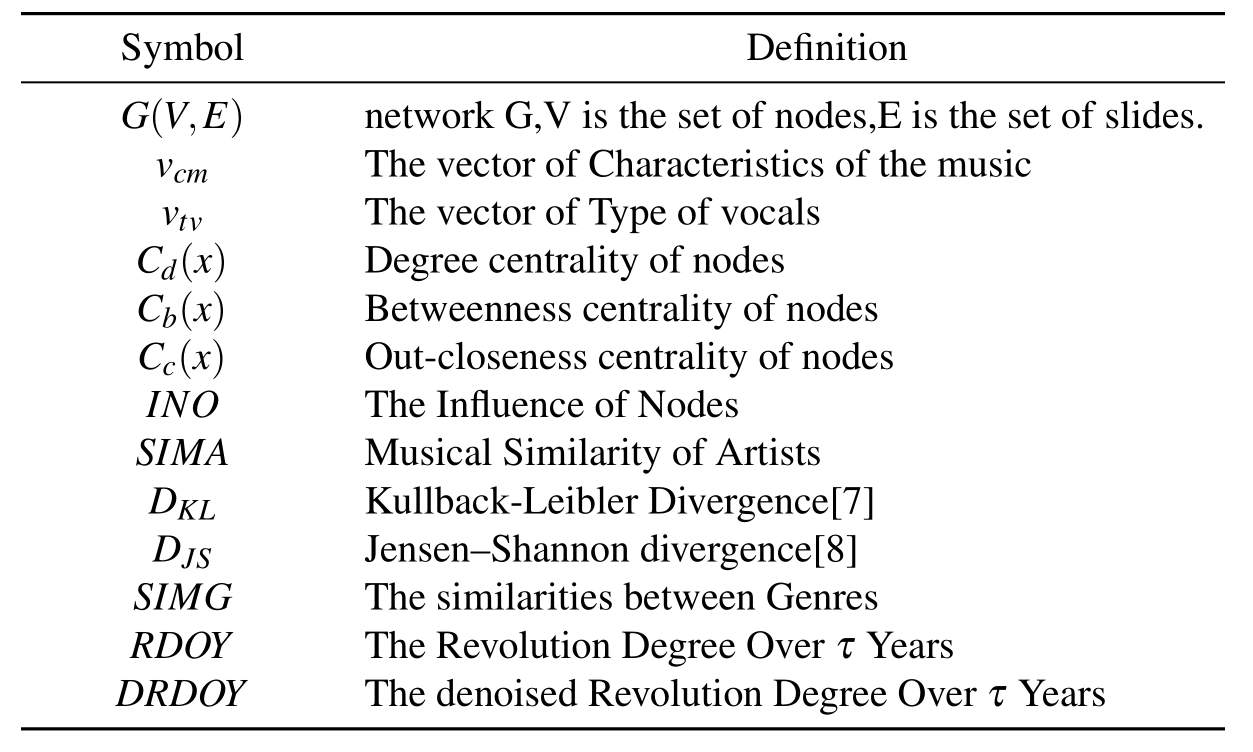
\includegraphics[width=3in]{./img/ttt}
	\caption{Simulation results for the network.}
\end{figure}
% \begin{table}[h]
% 	\begin{center}
% 		\renewcommand{\arraystretch}{1.3}
% 		\caption{Notations}
% 		\begin{tabular}{cl}
% 			\toprule
% 			\multicolumn{1}{m{3cm}}{\centering Symbol}
% 			&\multicolumn{1}{m{8cm}}{\centering Definition}\\
% 			\midrule
% 			$G(V,E)$&network G,V is the set of nodes,E is the set of slides.\\
% 			$v_{cm}$&The vector of Characteristics of the music \\
% 			$v_{tv}$& The vector of Type of vocals\\
% 			$C_{d}(x)$&Degree centrality of nodes\\
% 			$C_{b}(x)$&Betweenness centrality of nodes\\
% 			$C_c(x)$&Out-closeness centrality of nodes\\
% 			$INO$ & The Influence of Nodes\\
% 			$SIMA$&Musical Similarity of Artists\\
% 			$D_{KL}$&Kullback-Leibler Divergence\cite{7}\\
% 			$D_{JS}$&Jensen–Shannon divergence\cite{8}\\
% 			$SIMG$&The similarities between Genres\\
% 			$RDOY$&The Revolution Degree Over $\tau$ Years\\
% 			$DRDOY$&The denoised Revolution Degree Over $\tau$ Years\\
% 			\bottomrule
% 		\end{tabular}\label{tb:notation}
% 	\end{center}
% \end{table}

\section{TASK 1:Building Network}

\subsection{The Model 1:Influencer and Follower Network}

\begin{figure}[t]
	\centering
	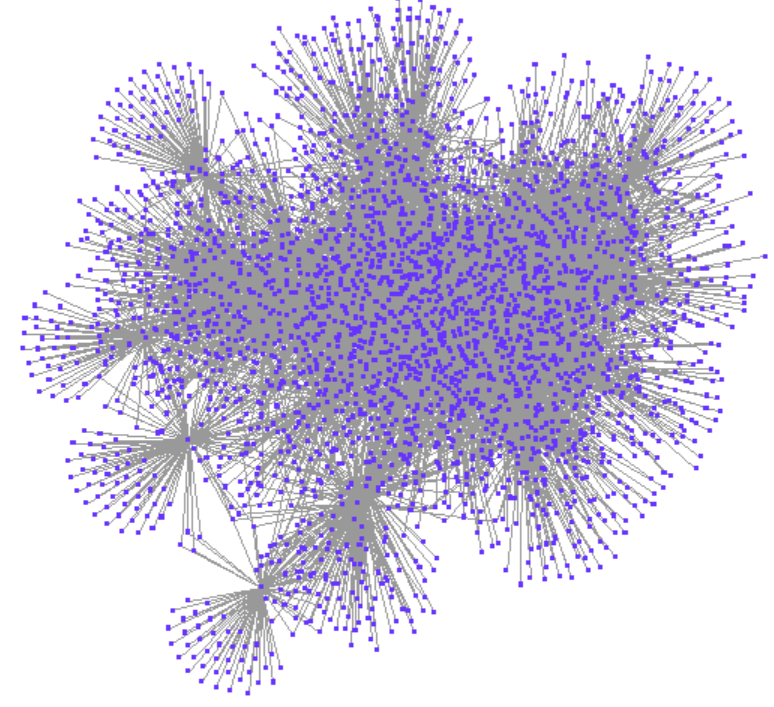
\includegraphics[width=2.5in]{./img/large_network}
	\caption{Simulation results for the network.}
\end{figure}
The relationships between influencers and followers in the data are real and measurable. Based on the information given in the title, the relationship between the influencer and the follower is collected from the artist himself, we can almost believe that the influence exists, and that there is a measure to measure the influence;

The influence of musical artists is irreversible. In fact, only early musicians can influence later artists.

Musical artists are active for a period of 10 years. Based on the data provided, we can only judge the approximate time period during which the artist began his musical career, however, we reasonably believe that this sums up a considerable part of the musician’s musical career. Moreover, because the influence between musicians is mainly expressed through works, the correlation with the musicians’active time is not very strong.

The style of a musical artist’s music is equivalent to that of a musician. Because of the limitations of the data, the characteristics of artists can only be inferred from the statistics of their music.

The work of a musical artist can reflect the influence of musical artists. Different artists create music with different styles, through the observation of the characteristics of the works, can measure the artists direct specific impact.

\begin{figure}[htbp]
	\centering
	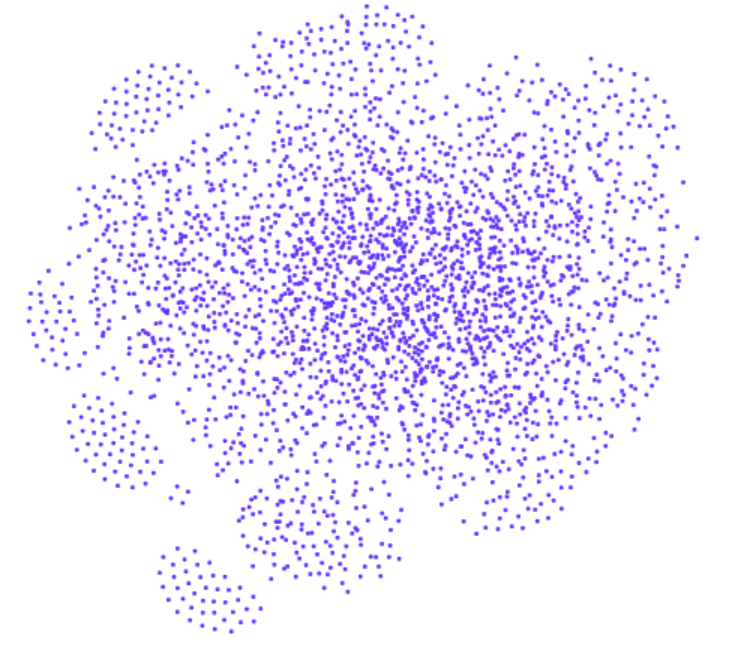
\includegraphics[width=.3\textwidth]{./img/large_network1}
	\caption{The network}\label{fig:network}
\end{figure}
\begin{figure}[htbp]
	\centering
	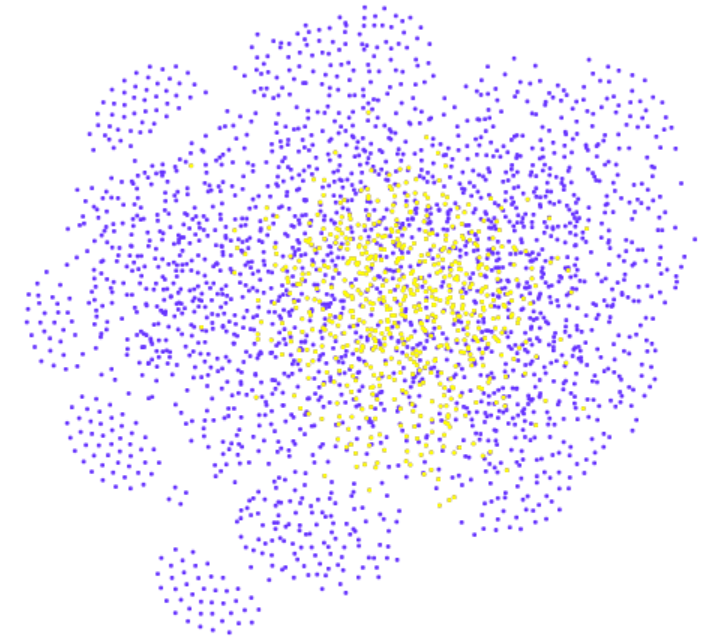
\includegraphics[width=.3\textwidth]{./img/large_network2}
	\caption{The network}\label{fig:network}
\end{figure}
\subsection{Measure Music Influence of Artist}
In graph theory and network analysis, Centrality is an indicator of the importance/influence of nodes in a network. In social network analysis, a basic task is to identify which people in a group are more influential than others, thus helping us to understand their role in the network.\\
We divide the influence of network nodes into three parts and give the corresponding measures:

\textbf{Number of followers:} measured by Degree Centrality. Take the corresponding node as the influencer and count the number of its followers. The more followers, the more influence.

\textbf{Importance in the transmission of musical art:} measured by Betweenness Centrality. Since the influence of artists is irreversible in time, good works of art need to be inherited and carried forward, we should consider the role of artists in the process of inheriting the essence of music. The mediating centrality of a node quantifies the number of shortest paths through the node, which is the number of times that one node acts as the bridge of the shortest path between two other nodes, and the mediating centrality of one node is higher, it means that many or even all of the shortest paths between other points must pass through it. Intermediary centricity is a good description of the influence network in the “Transmission”of the role of the hub.

\textbf{The historical position of the artist:} measured by Out-closeness Centrality. Clearly, the artist’s place in history can not be ignored. The network of influence of artists is obviously similar to the “Tree”network, the oldest few artists act as a few “Trunk”role. The near-centroid of the node computes the reciprocal sum of the shortest path lengths to the other nodes. A good approximation of the “Trunk”on each “Leaf”influence-the number of leaves and far and near.
\begin{itemize}
	\item Degree centrality
	\[C_d(x)=\sum_{i=1}^{n}a_{xi}\]
	Where $x$ is the influencer, $n$ is the total of nodes in a network, $a_{x,i}$ is a variable indicating whether the influencer $x$ connected with the node i or not. $a_{ix}=0 or 1$ in the directed network.
	
	\item Betweenness centrality
	\[C_b(x)= \sum_{i=1}^{n}\sum_{j=1}^{n}{l_{i,j}(x)}\]
	$l_{i,j}(x)$is if the shortest path from $i$ to $j$ goes through $x$;
	
	\item Out-closeness centrality
	\[ c_c(x)= \sum_{i=1}^{n}\frac{1}{dist(x,i)} \]
	$dist(x,i)$discribes the distance from node $x$ to node $i$,values $[0,\infty)$
\end{itemize}
A combination of these three characteristics provides a good measure of the Influence of Nodes:
\begin{equation}\label{eq:similarity of nodes}
ION(x)= \frac{C_d (x)}{max C_d (x)} +\frac{C_b (x)}{max C_b (x)}+\frac{C_c (x)}{max C_c (x)}
\end{equation}
\subsection{Explore and Describe subnetwork}
We went from 1930 to 1950, all artists, to build our subnetwork, which fully reflects the relationships among musicians, and is enough to tap into some early musical expression.
We have calculated the degree distribution of the nodes in the subnetwork. It is found that most nodes have lower degrees and a few nodes have higher degrees. If the probability distribution $p (k)$ of degree of nodes is used to denote the frequency of occurrence of nodes of degree k in a network, the following concise formula is used:
\[p(k)\backsim k^{-\gamma}\]
According to scientists’research on social networks, the influence transfer network is also a kind of social network, for many complex networks in the real world, such as the Internet, social networks, etc. , the number of connections (degrees) that each node has follows a power-law\ref{fig:exp} distribution. In other words, most artists are unknown, and a few artists have great influence over one another.
\begin{figure}[htbp]
	\centering
	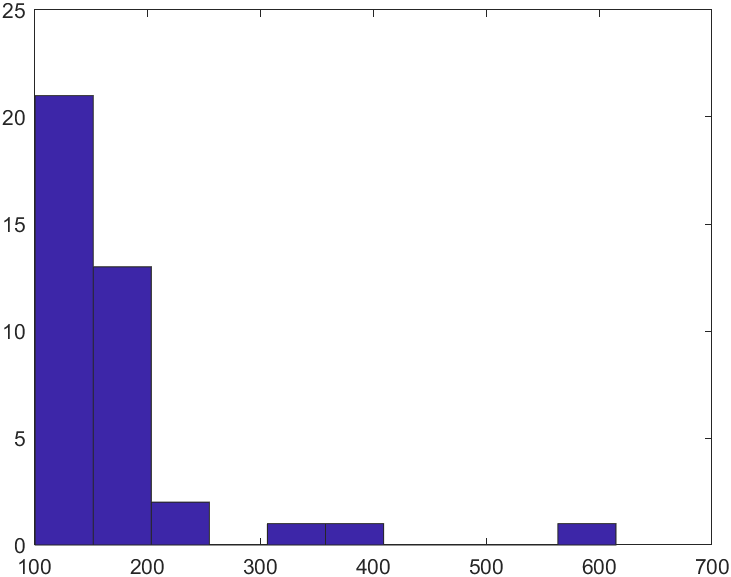
\includegraphics[width=.3\textwidth]{./img/exp}
	\caption{The power-low distribution of degrees}\label{fig:exp}
\end{figure}

According to the nature of the nodes, we advance the different years of the network nodes, we found that in the early period of the development of music, The Country genre artists number the most, the most prosperous. The most influential artists of the genre are Hank Williams, which indicates that they were the founders and pioneers of the early 6 genres(Country,Vocal,Blues,R\&B,Folk,Jazz); the Folk genre has the fewest artists and few artists.

\section{TASK 2:Measure similarity of Artists and Music}
\subsection{The Model 2:Measure Similarity Artists and Music}
Since both the artist and the music are external musical features, we can develop a measure of musical artist similarity based on their musical features.

\textbf{Data Engineering:}

we found that musical features are divided into two parts, “Character of Music”, which represents the track, and “Type of vocal,”which represents the sound of the piece, which should be taken into account. For the data set of full\_music\_data.csv, we have carried out a rigorous review and data screening, removed the illogical data, removed the mode and key features without distinction, and got five features respectively belonging to “Character of Music”and “Type of vocal”, then, according to the actual meaning of each feature, zero-mean normalization and Min-max normalization were performed. Considering whether more features may need to be reduced data dimension processing, we continue to carry out principal component analysis of the data. Principal component analysis (PCA) is a common method for dimensionality reduction. PCA replaces the original N features with fewer M features and new M features, while maximizing sample variance and ensuring independence. According to the principle of principal component analysis (PCA) , we calculated the KMO value of the data, which is a measure of PCA, and found that the KMO value is less than 0.6, so it is not suitable for dimension reduction. Therefore, we try to preserve the original features as much as possible, standardize the data, and then construct a similarity between the artist and the music.

We construct vectors for two types of features:
The vector of Characteristics of the music, A certain artist $x$:
\[v_{cm}(x)=(c_1(x),c_2(x),\ldots,c_m(x))\]
Where $m$ is the dimension of feature and it's value is equal to 5  in this model. \\
The vector of Type of vocals:
\[v_{tv}(x)=(v_1(x),v_2(x),\ldots,v_n(x))\]
Where $n$ is the dimension of feature and it's value is equal to 5  in this model.\\
To measure Musical Similarity of Artists($SIMA$) , we choose:cosine similarity

\begin{equation}\label{eq:Simlarity of music}
	\begin{aligned}
		& SIMA(x,y)\\
		& =0.7\times cos<v_{cm}(x),v_{cm}(y)>\\
		& + 0.3\times cos<v_{tv}(x),v_{tv}(y)>
	\end{aligned}
\end{equation}

where $<,>$ represents the vector angle,SIMA values from -1 to 1.

Vector similarity can be well measured by measuring the angle between two vectors. Cosine distance is more embodied in the overall difference of music features, the evaluation of music vector features of the relative size. When the two vectors are parallel, the similarity is 1; when the two vectors are opposite, the similarity is-1; when they are perpendicular to each other, the similarity is 0. After analyzing the meaning of each feature, we think that the importance of music is expression, better appeal to the audience, the way sound is not so important. We attach more importance to the similarity of “Character of Music”and think that the characteristics of Music track are more important.
\subsection{Compare Similarity between Artist and Music}
Intra-genre and inter-genre artist similarity refers to the overall, intra-genre and inter-genre artist who is more similar, should statistics within the genre and inter-genre so that the average value of individual similarity, compare the size. However, when the sample size is too large, due to the number of artists, the statistical complexity is difficult to achieve, we use a random sample of some individuals to compare the similarity. Based on the law of large numbers, this is a reasonable way to estimate the similarity of artists within and between genres.

We picked Pop/Rock and The Rolling Stones, The Byrds and Cream, The Stooges
And Kraftwerk, for each genre, randomly selected 100 artists and calculated the average similarity within and across genres. The average similarity of artists within a genre is 0.25, and that of artists across genres is 0.13, taking into account the range of similarity $[-1,1] $ , we think that the similarity between the artists within the genre is obviously greater than the similarity between the artists within the genre.

\section{TASK 3:Similarities, Influences and Distinguish of Genres}
\subsection{The Strong Model 3: Measure Similarities and Influences between and within Genres}
We believe that a simple consideration of each genre’s songs and writers’styles can not fully reflect the characteristics of the genre, but should also take full account of even the same genre, a musical feature is not a more certain measure. We count the characteristic distribution of this genre music, we can judge the performance and characteristics of this genre more comprehensively.

In order to reduce the computational complexity, we combine the actual meaning of the data with the P value test of the data, we screen out the more useful and important 10 features , 5 is 'characteristics of music', 5 come from 'Vocal of Type', and since we think that the former is more differentiated than the latter, we impose a different importance ; these characteristics come from the performance of the genres that can be well measured. After the data statistics, for every genre k, get 10 different distributions of 10 characteristics.
\[p_k=(p_k(x_1),p_k(x_2),\cdots,p_k(x_{10}))\]
\begin{figure}[htbp]
	\centering
	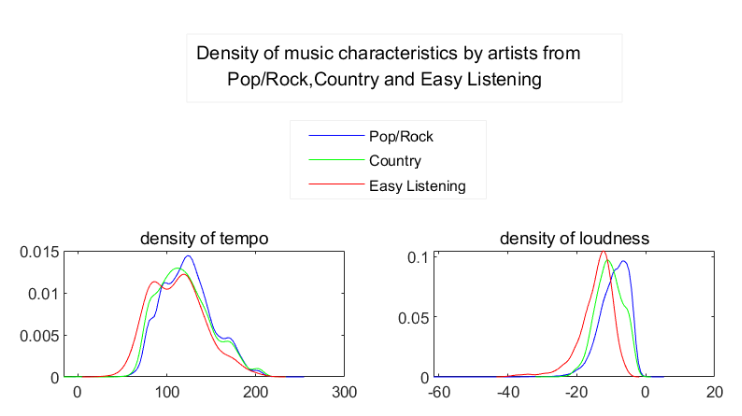
\includegraphics[width=.4\textwidth]{./img/density}
	\caption{The density of three genres and two characteristics}\label{fig:density}
\end{figure}

The Distribution of Genres over time show follow:\\
\begin{figure}[h]
	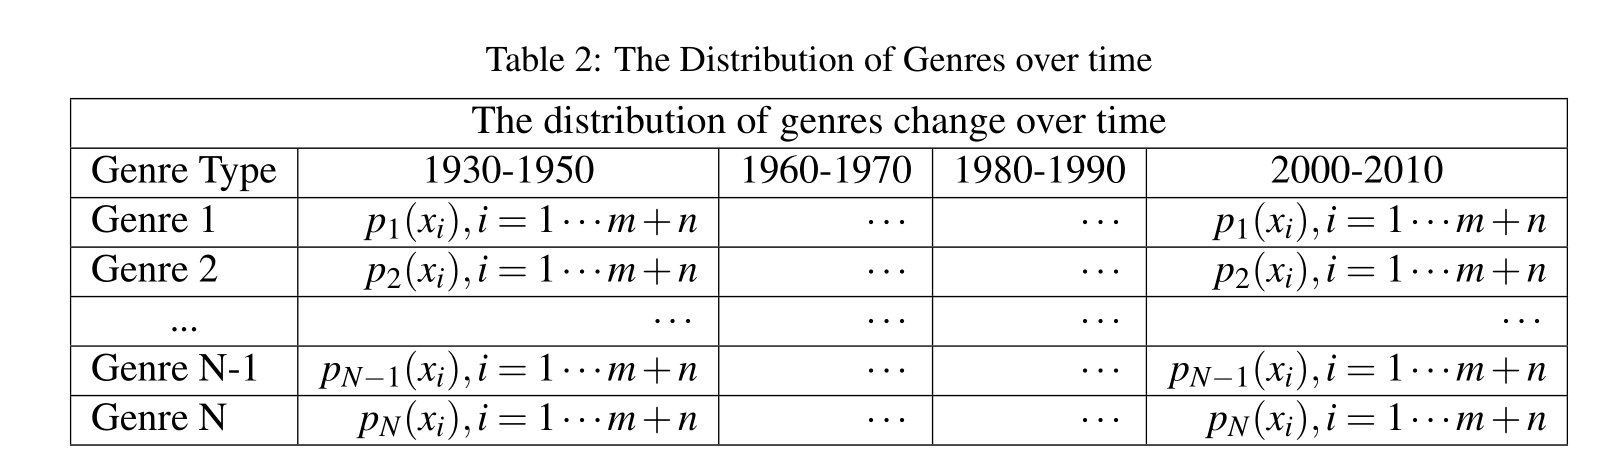
\includegraphics[width=.52\textwidth]{./img/qqq.png}
	\caption{The Distribution of Genres over time}
\end{figure}
% \begin{small}
% 	\begin{small}
% 		\begin{table}[!htbp]
% 			\centering
% 			\caption{The Distribution of Genres over time}
% 			\begin{tabular}{|l|r|r|r|r|}
% 				\hline
% 				\multicolumn{5}{|c|}{The distribution of genres change over time} \\
% 				\hline
% 				Genre Type & \multicolumn{1}{c|}{1930-1950} & \multicolumn{1}{c|}{1960-1970} & \multicolumn{1}{c|}{1980-1990} & \multicolumn{1}{c|}{2000-2010} \\
% 				\hline
% 				Genre 1 &    $p_1(x_i),i=1\cdots m+n$   &   $\cdots$    &   $\cdots$    & $p_1(x_i),i=1\cdots m+n$ \\
% 				\hline
% 				Genre 2 &    $p_2(x_i),i=1\cdots m+n$   &    $\cdots$   &   $\cdots$    & $p_2(x_i),i=1\cdots m+n$ \\
% 				\hline
% 				\multicolumn{1}{|c|}{...} &   $\cdots$    &   $\cdots$    &   $\cdots$   & $\cdots$ \\
% 				\hline
% 				Genre N-1 &   $p_{N-1}(x_i),i=1\cdots m+n$    &    $\cdots$   &  $\cdots$    & $p_{N-1}(x_i),i=1\cdots m+n$ \\
% 				\hline
% 				Genre N &    $p_N(x_i),i=1\cdots m+n$   &   $\cdots$   &  $\cdots$    & $p_N(x_i),i=1\cdots m+n$ \\
% 				\hline
% 			\end{tabular}%
		
% 			\label{tb:The Distribution of Genres over time}%
% 		\end{table}%
% 	\end{small}
% \end{small}
In statistics, KL divergence can be used to measure the difference between the relative distributions of $P (x) $and $q (x) $. If the two branches are identical, KL Divergence value is 0 and the maximum value of distribution difference is 1.The detail can be described by equation:
\begin{equation}\label{eq:KL}
	\begin{aligned}
		D_{KL}(p||q)
		&=\sum_{x}p(x)\ln q(x)-\sum_{x}p(x)logp(x)	\\
		&=\sum_{x}p(x)\ln\frac{p(x)}{q(x)}
		\end{aligned}
\end{equation}
\[D_{KL}(p||q)\neq D_{KL}(q||p)\]
In order to measure the difference between the two distributions, JS divergence is proposed\cite{bullmore2009complex}, which can measure the difference between the two distributions and has symmetry.
The detail can be described by equation:
\begin{equation}\label{eq:JS}
D_{JS}(p,q)=\frac{1}{2}( D_{KL}(p||\frac{p+q}{2})+D_{KL}(q||\frac{p+q}{2}))\\
\end{equation}
\[D_{JS}(p,q)= D_{JS}(q,p),D_{JS}(p,q)\in [0,1] \]
The above measures can be applied to the distribution of a feature in a genre, and can be used to measure the difference between any two distributions.
If we apply the calculation of JS divergence to the distribution of two characteristics $x_i,x_j$ of two genres, we can get the similarity of two characteristics $x_i,x_j$ between two genres:
\begin{equation}\label{eq:SIMG 1}
	\begin{aligned}
		SIMG_{k,l}(i)&=SIMG[p_k(x_i),p_l(x_i)]\\
		&=1-D_{JS}[p_k(x_i),p_l(x_i)]
	\end{aligned}
\end{equation}
The similarities between genres $k, l $
\begin{equation}\label{eq:SIMG 2}
	\begin{aligned}
		SIMG_{k,l}&=SIMG(p_k,p_l)\\
		&=1-\frac{1}{m+n} \sum_{i=1}^{m+n} D_{JS}[p_k(x_i),p_l(x_i)]
	\end{aligned}
\end{equation}
\subsection{Compare Similarity and Influence of Genres}
The influence of genre refers to the influence of each genre on the genre, including four kinds of influence relations: the influence of the same genre, the influence of the earlier genre on the later genre, the influence of one genre on the other genre, and the influence of other genres on this genre; Between the other schools of thought.

Since we have established a bi-attribute directed network, we can divide the network graph into sub-networks which are not contained by each other. A good assessment of the influence relationships between/within genres. Taking all the nodes of each genre as a whole, we can also get the degree and the degree between the genres. These two parameters directly measure the external influence of the genre and the number of external influence received, it’s a good measure of genre influence.

\[Out_{degree}(i)=\sum_{x\in \Gamma_i \ and\  y\notin \Gamma_i}a_{xy}\]
\[In_{degree}(i)=\sum_{x\in \Gamma_i \ and\  y\notin \Gamma_i}a_{yx}\]

$a_{x,y}$ is whether $y$ influenced by $x$, values 0 or 1,$\Gamma_i$ is the nodes set of genre i.
We take the Pop/Rock genre as an example to compare its impact on other genres Figure \ref{fig:result_pop_out}
First, calculate the degrees of all the nodes within the genre, measure the meaning of the transmission and communication of artists within the genre, we get
The first three genres of internal influence: Pop/Track, R \& B, country; show that their music genres have a wider audience and a larger number of artists within the genres, making it easier to convey influence.
The two genres with the lowest in-house influence are Avant-Garde, Children’s, which suggests not only that there are fewer artists but also that there is less continuity between them, considering that they are less popular and less diffusive.

\begin{figure}[htbp]
	\centering
	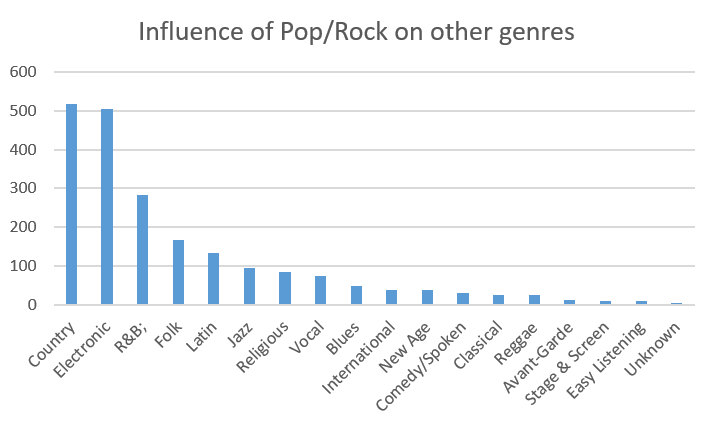
\includegraphics[width=.3\textwidth]{./img/influence_of_pop_on_others_1}
	\caption{The result of Task 3}\label{fig:result_pop_out}
\end{figure}

\subsection{Distinguish a Genre and Changing Process}
Around the genre Pop/Rock, we measured the most similar genre and the most disparate: Country and Easy Listening.

Their distribution for each feature is shown in the Figure below.

we determine that genre Pop/Rock and genre Country are very similar in Valence, tempo, mode, liveness, speechiness, duram;
We identified the differences between genre Pop/Rock and genre Easy Listening in terms of danceability, energy, key, Valence, etc.

Based on the calculation of similarity and the distribution of features, we can easily explain the differences between schools.
\begin{figure}[htbp]
	\centering
	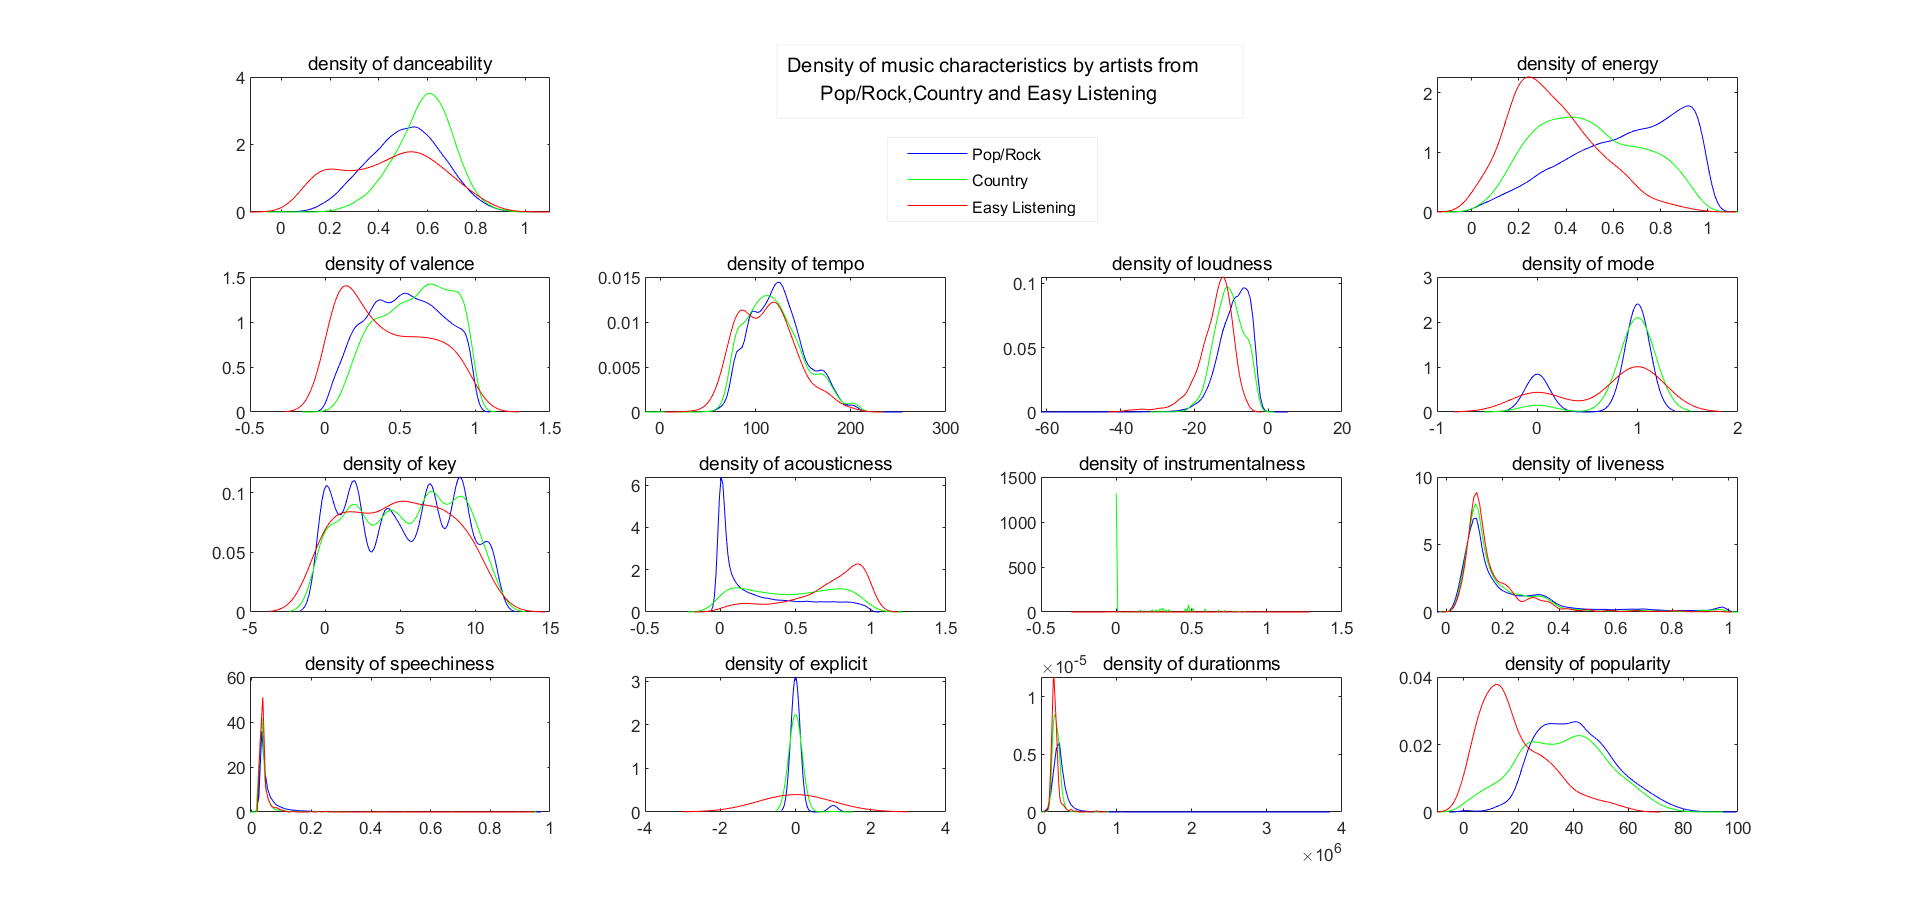
\includegraphics[width=.5\textwidth]{./img/pop_coutry_easy}
	\caption{Three genres distinguish}\label{fig:pop_country_easy}
\end{figure}
At the same time, we can also get the most similar of the different schools, we guess that these schools, the later schools may be affected by the earlier schools.

When we look at the distribution, of a genre feature $x_j$ over time, we can also see that the same genre, has evolved over time, not just in terms of numerical features.
\section{TASK 4:Testing Influence and Find Characteristics}
\subsection{Indicate the Factuality of Influence}
Consider whether the influence of musicians on each other can be expressed in terms of cosine similarity of musical features($SIMG(x,y)\eqref{eq:Simlarity of music}$). We know that if a musician has a profound influence on another musician, we usually think of it as having an influence on the musical character of the artist. The deeper the influence, the closer the similarity of the musician’s features to 1 OR \-1, the more likely it is to inherit the musical style, or to reform it. The effect could be the effect of a trait, like tempo, or it could be the effect of all the traits combined.

In order to determine the benchmark that can prove the influence is real, we calculate the average similarity between any two artists by random sampling, that is, the most likely similarity between artists, whether the influence is real or not -- the benchmark. Again, using statistical theory, we can think of musical similarity as a random variable, when there are enough musicians, and there are enough influence relationships between musicians, to ignore the influence goals given by the affected people. Then, according to the law of large numbers, we select enough musicians at random, calculate the average value of similarity, and can reasonably estimate the expectation of similarity -- the benchmark of similarity.
We renamed it the benchmark similarity a% .

When the follower gives the goal of the influencer, I calculate the similarity between the influencer and the follower. If the similarity between the influencer and the follower is obviously larger or smaller than the benchmark similarity, then there is good reason to think that the influence is real Even by comparing the musical features of two artists, we can know the specific content of the influence relationship.

A random sample of 400 artists was randomly divided into 200 pairs, and the average similarity of each pair was calculated to be 9.6\% -- the benchmark similarity; this data can represent the general similarity, that is, the similarity estimate when it is uncertain whether there is an effect; If the similarity between two individuals is obviously greater than 9.6\% or obviously less than 9.6\% , the influence relation is considered to be obvious; if it is close to 9.6% , the influence relation is not sure.

A further sample of 100 was used to calculate an average similarity of 18.4\% between known influencers and those affected; there was a significant difference between the two, and we considered that the given influence relationship really existed. But the degree of influence is not high. We speculate that the artist’s influence is mainly positive, and the similarity is greater than 0. But some of the influence between the influencer and the follower is opposite -- innovation, the similarity is less than 0, and the average value is offset by positive and negative values.
\subsection{More Contagious Music Characteristics}
The development of music stems from the pursuit of richer, more diverse, and more beautiful music, and a musician is committed to making more popular music, regardless of genre.
Statistically, Energy, loudness, robustness and popularity had a greater correlation, all close to 0.5. We think these traits are more contagious.

\section{TASK 5:Identify Characteristics signifying Musical revolutions}
\subsection{Characteristics Classification and Dimension Reduction}
To measure the evolution of music, we started with: Data by year Data, and since we are looking at music Data from year to year, the correlation between musical characteristics is even more pronounced. According to the interpretation of music (Track) and real data, there is a strong correlation between loudness, tempo and energy, while dance ability requires a combination of tempo/rhythm/beat strength, these characteristics are clearly related to the energy/loudness of music. We will use this to reduce the dimension of the data, in order to more intuitive observation of the evolution of features.

Therefore, we reduced the principal component dimensions of five characters belonging to ‘Character of Music’to generate two principal components (PC, Y) , with an interpretation rate of variance of 89\% , named:
\begin{itemize}
	\item Ability of infection constituent-- generalize the Ability to interact with the audience;
	\item Ability of positivity constituent -- the positive meaning of music.
\end{itemize}
The principal component analysis (PCA) was also used to reduce the dimension of Type of Vocal, and three principal components (PC, Z) were extracted. The explanation rate of variance was 90\%
\begin{itemize}
	\item The Vocal constituent -- All the Type of vocal characteristics are summed up evenly
	\item The Music language constituent -- representing the linguistic aspect of Music;
	\item The liveness constituent -- representing whether or not Music is focused on live performance.
\end{itemize}

\begin{figure}[!htbp]
	\centering
	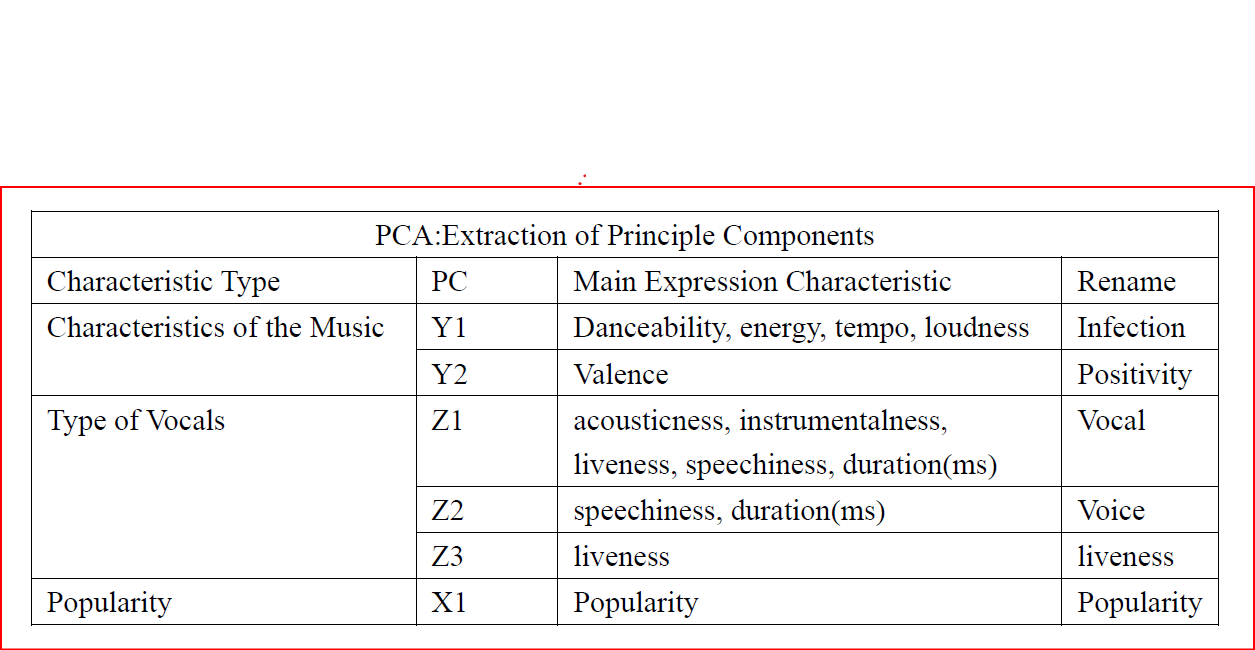
\includegraphics[width=.3\textwidth]{./img/table_of_component}
	\caption{The expression of components}\label{fig:table_of_component}
\end{figure}

\[v^{t}=(y_1^{t},y_2^{t},z_1^{t},z_2^{t},z_3^{t},x_1^{t})\]

\subsection{Measure Musical Revolution}
This can be due to a sequence of small changes, a cooperative effort of artists, a series of influential artists, or a shift within society. In order to highlight the more obvious changes, we create a time-smoothed degree of change based on the cosine similarity model -- not only is it a good measure of how much the genre has changed, but it is also an effective measure of how little it has fluctuated, intuitively and rationally extrapolate the timing of major changes. The bigger the change, the smaller the measure of change; the smaller the change, the bigger the measure of change.

The Revolution Degree Over $\tau$ Years:
\[
RDOY(t)=cos<v^{t},v^{t+\tau}> \\
=\frac{v^{t} \cdot (v^{t+\tau})^{T}}{{\|v^{t}\|}_2 \cdot {\|v^{t+\tau}\|}_2}
\]

The Denoised Revolution Degree Over $\tau$ Years:
$$
\begin{aligned}
& 	DRDOY(t)\\ 
& 	=\frac{1}{5}(RDOY({t-2})+RDOY({t-1})+RDOY({t})\\
& 	+RDOY({t+1})+RDOY({t+2}))
\end{aligned}
$$
\begin{figure}[!htbp]
	\centering
	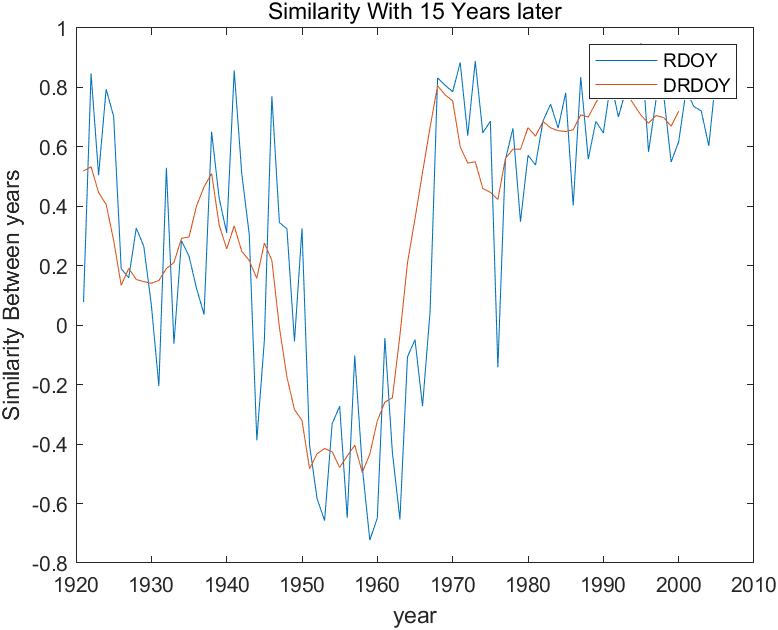
\includegraphics[width=.3\textwidth]{./img/revolution}
	\caption{The result of Task 5}\label{fig:revolution}
\end{figure}


\subsection{The Revolution Decades and Revolutionaries}
We found that influencer and follower had an average influence time interval of 15 years, and we took time interval $\tau = 15$, it shows that the artists in this period were very different from the music styles 15 years later, and identified the time when the revolution took place.

We calculated the relative Degree of Revolution of the five musical components according to the principal component’s explanation of the different characteristics of the music.
\[\frac{v_{i}^{t+\tau}-v_{i}^{t}}{v_{i}^{t}} \times 100\%\]
% Table generated by Excel2LaTeX from sheet 'Sheet1'
\begin{table}[!htbp]
	\centering
	\caption{The Revolution Decades($\%$)}
	\begin{tabular}{c|cccccc}
		\hline
		Periods& Infective& Positive & Vocal & Voice &Liveness & Popularity \\
		\hline
		$1930-1945$ & $-135$  & $106$   & $3$     & \textcolor{red}{$-519 $} & $-131$  & $-3$ \\
		$1960-1975$ & $-144 $ & \textcolor{red}{$-1235$} & \textcolor{red}{$445$}   & $-303$  & $-206$  & $-185$ \\
		\hline
	\end{tabular}%
	\label{tb:The Revolution Decades}%
\end{table}%
By comparison, the content of Voice in music from 1930 to 1945 was greatly reduced, which indicated that the music style began to change to singing-based music, greatly reduced the proportion of instrumentality, and the music conveyed more positive emotion
The 1960-1975 musical style had a 10-fold reduction in positivity, suggesting that the sound more negative (e. g. sad, depressed, angry). All this has led to a dramatic change in musical style.

\begin{figure}[htbp]
	\begin{minipage}[t]{0.5\textwidth}
		\centering
		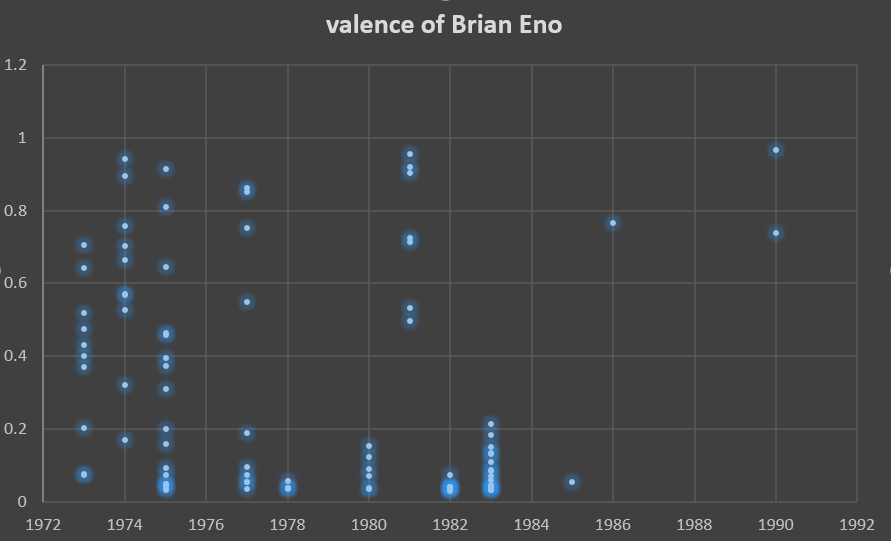
\includegraphics[width=.3\textwidth]{./img/valence_of_Brian}
		\caption{Valence of Brian\label{fig:valence_of_Brian}}
	\end{minipage}
	\qquad
	\begin{minipage}[t]{0.5\textwidth}
		\centering
		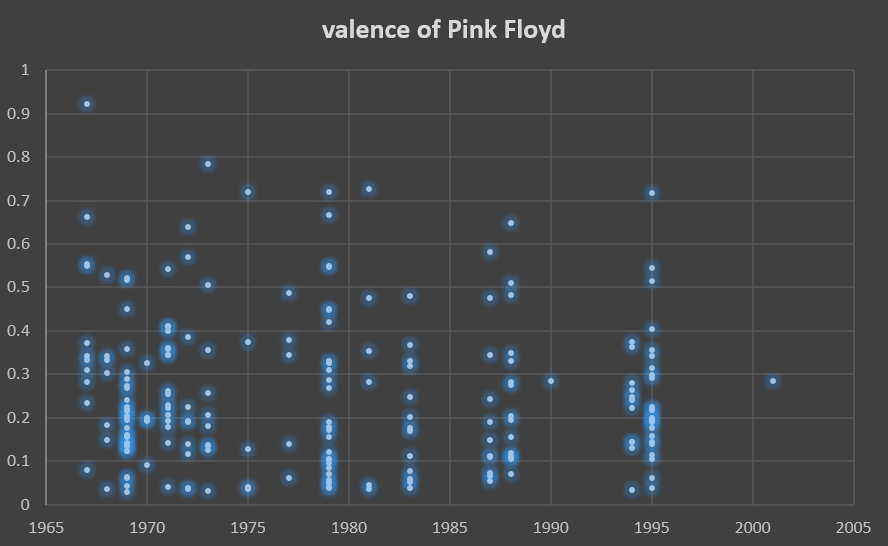
\includegraphics[width=.3\textwidth]{./img/valence_of_PinkFloyd}
		\caption{Valence of PinkFloyd\label{fig:valence_of_PinkFloyd}}
	\end{minipage}
\end{figure}
\textbf{Revolution:}

\textbf{1930-1945:} Hank Williams and Miles Davis were the two artists who led the revolution in the 1930s and 1940s.

\textbf{1960-1975:} Brian and Pink Floyd were two of the most revolutionary artists of the 1960s and 1970s.

Valence is a measure describing the musical positiveness conveyed by a track. A value of 0.0 is most negative and 1.0 is most positive. Tracks with high valence sound more positive (e.g. happy, cheerful, euphoric), while tracks with low valence sound more negative (e.g. sad, depressed, angry).

We count all the works of the artist Pink Floyd from 1967 to 2001, and draw a scatter plot of each work Valence. Most of the works have a Valence value of less than 0.5 Despite his influence, artist Brian’s work has been intense since 1974, at the end of the music revolution.
\section{TASK 6:Identify dynamic and Changing over time}
\subsection{Analyze the influence processes of musical evolution}
The development of music genre is influenced by many factors, which can not only inherit and carry forward the features of this genre, but also absorb the features of other genres, including the way of playing, tune and singing. The various features of different genres of music are fused with each other, and the music artists themselves are constantly seeking richer and more varied music. The small influence of each artist and the whole society’s pursuit of different styles of music are likely to result in a dramatic change in the characteristics of a genre.

In addition, the evolution of musical genres may be influenced by social development. With the development of American industrialization, the economy became more and more prosperous as early as the 19th century, and people’s material living standard was greatly enriched. People’s material standard of living has been greatly enriched, people put forward new request to music art continuously, urge artists to walk out the road of open innovation, want to make music face the public.

We need to measure the impact process of a genre, and in order to simplify the model, we now consider only the interaction between genre and genre/musicians within genre. We see the interaction of artists as the main driving force behind the evolution of the genre. In order to study the influence process of a genre over time, we will rationally quantify the influence process of a genre based on the influence network of musicians.

First, the difference in influence. We take Pop/Rock, and in the network of influence, the influence of the Pop/Rock genre can be divided into four parts: the influence of the early Pop/Rock artists on the later Pop/Rock artists, the influence of other Pop/Rock artists on the later Pop/Rock artists, the influence of the Pop/Rock genre on the later Pop/Rock genre, and the influence of the Pop/Rock genre on the later Pop/Rock genre. There are four kinds of influence processes in each genre at the same time. Some influence promotes the inheritance of the genre and keeps the genre in its original style; some influence promotes the change of the genre, as Pop/Rock continues to absorb the singing/accompaniment/composition features of other genres, the Pop/Rock genre will change. Sometimes the impact of both will be slow and subtle, and sometimes it will lead to rapid change because of the power of certain genres.

\subsection{The Genres' Changing over Time}
On the basis of the above analysis, we define the influence transmission mode. In graph network, because each node has only one time attribute, different time corresponds to different nodes. We use $V_{PR}(t)$ to represent the set of nodes corresponding to the Pop/Rock genre at time t, $V(t) \verb|\| V_{PR}(t)$ represent the set of nodes corresponding to other genres, and use $ E\{A,B\}$ to denote the number of edges from the set A to the set B with directivity, get Four measures of impact:
\begin{figure}[!htbp]
	\centering
	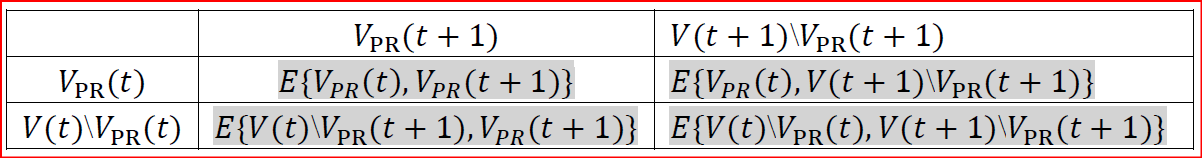
\includegraphics[width=.3\textwidth]{./img/task6}
	\caption{The result of Task 6}\label{fig:task6}
\end{figure}

We study the change of instrumentalness from fullmusic data in four periods:$1920-1929,1930-1939,1940-1949,1950-1959$.A point in the chart represents a song.

\begin{figure}[htbp]
	\begin{minipage}[t]{0.5\textwidth}
		\centering
		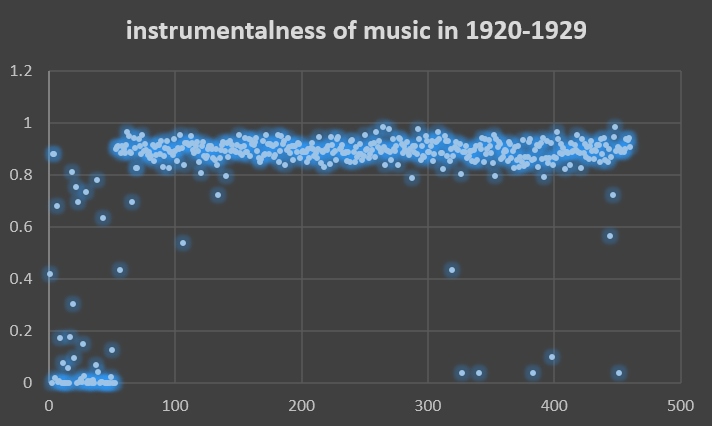
\includegraphics[scale=0.5]{./img/instrumentalness_of_music_in_1920_1929}
		\caption{instrumentalness of music in 1920-1929\label{fig:instrumentalness1}}
	\end{minipage}
	\begin{minipage}[t]{0.5\textwidth}
		\centering
		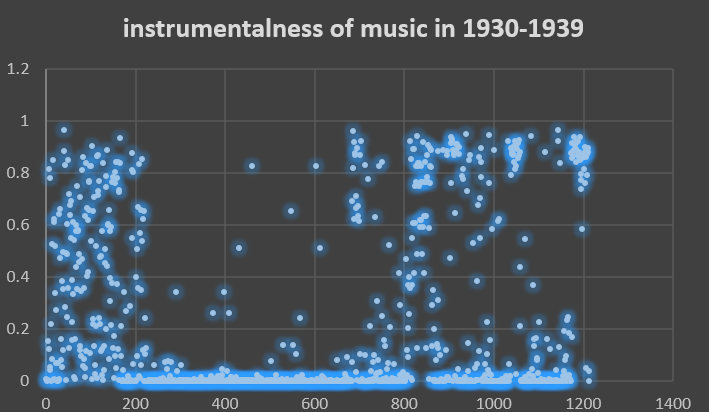
\includegraphics[scale=0.5]{./img/instrumentalness_of_music_in_1930_1939}
		\caption{instrumentalness of music in 1930-1939\label{fig:instrumentalness2}}
	\end{minipage}
	\qquad
	\begin{minipage}[t]{0.5\textwidth}
		\centering
		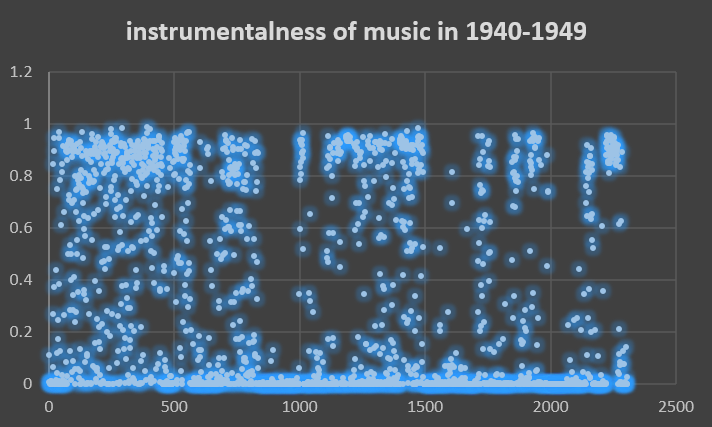
\includegraphics[scale=0.5]{./img/instrumentalness_of_music_in_1940_1949}
		\caption{instrumentalness of music in 1940-1949\label{fig:instrumentalness3}}
	\end{minipage}
	\begin{minipage}[t]{0.5\textwidth}
		\centering
		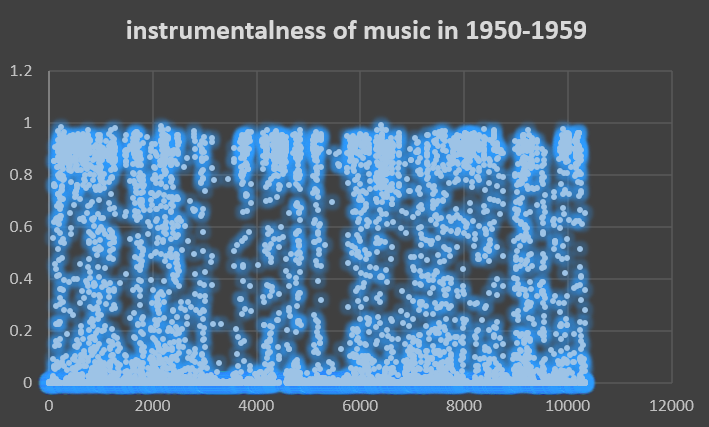
\includegraphics[scale=0.5]{./img/instrumentalness_of_music_in_1950_1959}
		\caption{instrumentalness of music in 1950-1959\label{fig:instrumentalness4}}
	\end{minipage}
\end{figure}

In $1920-1929$,the level of instrumentalness is much high,but in $1930_1939$,the points move lower obviously and evidently. In the era coming later,instrumental ness relatively distributed evenly,having a large proportion of points gathering below $0.2$. This result is in accord with our findings above. It further vertifies that there is a music revolution in $1930-1945$ in which the instrumentalness became lower. After data processing,speechiness and duration in $1930-1945$ and valence in $1960-1975$ also have similar dramatic changes.
\section{TASK 7:Music and Society }

Music plays an important role in the collective human experience. Music in different periods can not only reflect people’s spiritual outlook in different historical periods, but also record people’s daily life and cultural background in different historical periods by music. When we look at the history of contemporary Western music, we are surprised to see the emergence of Native American musicians, from the academic John Cage to the Michael Jackson of pop music, its influence extends far beyond national borders and into every corner of the world. The content and form of the music itself has changed dramatically, with the amazing postmodern art and the crazy, passionate rock and roll performances that have revolutionized the way the world’s traditional music is created and appreciated, since its birth in the United States, contemporary music has been branded with the economic and political marks, playing an important role in the export of American culture and ideology.

Through the above analysis, with the change of the times, the artist’s creation has also changed. As for society and politics, the characteristics of songs in the era of peace and stability are different. The economic crisis, the Second World War, the Cold War, the scientific and technological revolution, and the rapid development of the Internet have a great influence on the development of music, music also plays a role in these historical events. The emergence of the Internet has influenced the form of music playing, especially the electronic music has a great influence on the traditional media such as the record player. The development of science and technology may also lead to differences in people’s interests in the field of music. The rise and fall of music genres are constantly changing with the change of historical periods. These changes are continuous, the boundaries between the prevailing genres of music are often blurred. The development of music interacts with the development of social, political, or technological change. We introduce the development of several major musical genres.

\textbf{ Bruce, music}
In the late 1920s and early 1930s, the United States experienced its first severe economic crisis, leaving much to be desired. Many black people moved from the rural south to the cities in order to survive. Black people gathered in the industrial cities in the hope of finding suitable jobs. By this time Bruce’s music was strong and vibrant, reflecting the feelings of the young black generation in urban life. Bruce’s music directly or indirectly influenced other forms of music, sowing the seeds for the development of other songs.

\textbf{Jazz music}
In 1921, with the release of the first all-black jazz album, jazz musicians by their own continuous exploration and innovation, get great development. Jazz appeals to a wide audience because it truly reflects the ethos and youthful energy of the American people, and because it is yet another way of communicating and expressing human emotions, and it’s more vivid and powerful than words. It expresses love, desire, anger, joy, and sorrow, as well as the vitality and freedom of the American people. Black Americans were a product of the prevalence of slavery, and jazz was the best way for black Americans to express their anger, their emotions, their creativity, their thoughts, their opinions, jazz, with its unique charm, is more easily understood and accepted than any other art form.

\textbf{Country music}
Thanks to the improvement of recording technology, country music brought endless comfort and hope to the American people during the Great Depression. After the rapid development in the 1950s, country music continues to grow. In the 1990s, country music entered another period of high tide, interwoven with other musical elements, showing unprecedented passion and vitality.

\textbf{Rock music}
After the Second World War, the Super Power Arms Race and the Cold War, the rapid industrialization and the severe ecological crisis, the world situation is full of Sleeper Cell and contradictions. People generally want to be able to vent something in their hearts, so that the injured mind to be comforted. Finally, in the field of art, rock music with an unprecedented momentum to ignite the fire in People’s hearts and swept the world. After the irrigation of the 1960s, it became one of the most important varieties of American music in the international market after World War II. Rock music is the concrete embodiment of the achievements of human culture and art. It is the first time that people’s thoughts, gratitude and connection are linked together. It makes people’s spirit and human culture get another leap.

\textbf{New Age Music}
After several scientific and technological revolutions, people have higher demands on music, and some musicians have integrated the concept of synthesizer sound into the way of acoustic performance or improvisation, which has inspired musicians to explore new fields. The 1980s saw the emergence of a new genre of music that was harder to define directly in terms of instrument type and style than in other musical styles, such as the New Age music, it’s more of a fusion of other genres. Especially after entering the 21st century, the level of urban modernization has been rapidly improved. Compared with the noisy cities, people begin to pursue the purity of mind, the harmony and stability of life, and the contents of New Age music are very rich, all the sounds of nature can be found in music.

With the development of electronic technology and communication technology, music songs in the 21st century are becoming more and more global. The styles of music during this period were also extremely rich and varied. Many songs have gone viral on the internet and have had a profound impact. Music from different regions collides to a higher level. In order to cater to the audience’s taste, different types of different styles of songs and singers emerge one after another.

\textbf{To sum up}, we can find that music after a century of development, different times have different characteristics. But no matter when, the popular music is close to the masses, most easy to arouse people’s heart resonance. Its creation is from the heart of the true feelings, can give our lives add gorgeous color, bring a lot of fun.
The influence of Bob Dylan and other singers on American culture.

\section{Conclusion}
\subsection{Strengths and Weaknesses}
\begin{itemize}
	\item We combine three metrics: Degree, Betweenness centrality, and Out-sensitivity centrality to measure the influence.
	
	\item We apply a new method better than cosine similarity. By means of random selection on artists, it is proved that artists within genres are similar than artists between genres.
	
	\item The distribution function of genre characteristics is innovatively proposed and the measurement of similar rows among genres with high adaptability and flexibility is constructed.
	\item Based on the similarity \cite{wu2020experimental} measure of music, the dynamic change degree of noise reduction is obtained, and the reasonable periods of music revolution are 1930-1945 and 1960-1975.
\end{itemize}



% 参考文献,此处以 MLA 引用格式为例
% \begin{thebibliography}{99}
% 	\bibitem{1} Einstein, A., Podolsky, B., \& Rosen, N. (1935). Can quantum-mechanical description of physical reality be considered complete?. \emph{Physical review}, 47(10), 777.
% 	\bibitem{2} \emph{A simple, easy \LaTeX\ template for MCM/ICM: EasyMCM}. (2018). Retrieved December 1, 2019, from\url{https://www.cnblogs.com/xjtu-blacksmith/p/easymcm.html}
	
% 	\bibitem{3} \url{https://en.wikipedia.org/wiki/Music_genre#cite_note-1}
% 	\bibitem{4} \url{https://en.wikipedia.org/wiki/Kullback\%E2\%80\%93Leibler_divergence }
% 	\bibitem{5} \url{https://blog.csdn.net/guoziqing506/article/details/51779536}
% 	\bibitem{6} \url{https://en.wikipedia.org/wiki/History_of_music}
% 	\bibitem{7}\url{https://en.wikipedia.org/wiki/Jensen\%E2\%80\%93Shannon_divergence}
% 	\bibitem{8}\url{https://en.wikipedia.org/wiki/Kullback\%E2\%80\%93Leibler_divergence}
	
% \end{thebibliography}
\bibliographystyle{IEEEtran}
\bibliography{ref}
\section{Appendix A}
	Given that the two problem data sets are limited to certain types and only some artists are considered, our work should be further deepened.
	Because our similarity-based measure has great richness and freedom, and the feature of describing network graph with distribution does not increase the computational complexity because of the size of data set, our model has tremendous advantages.
\begin{equation}\label{eq:SIMG 3}
	\begin{aligned}
	SIMG_{k,l}
	&=SIMG(p_k,p_l)\\
	&=1-\frac{1}{m+n} \sum_{i=1}^{m+n} D_{JS}[p_k(x_i),p_l(x_i)]
	\end{aligned}		
\end{equation}
	In addition, when we were doing the Data pre-processing, there weren’t enough 
	features, there were only 10 dimensions, so we couldn’t generalize the music information. 
	In fact, the number of musical features is far greater than the number of musical features given. 
	We can’t describe musical similarities, changes, and evolution very well with limited information, 
	so more data is helpful. If enough features are considered, we plan to use principal component analysis (PCA) to reduce data dimension and fully mine the information of data. We plan to extend the network model.
	
	As for the study of the influence of music on culture, we consider the study of culture-related features and further analysis, such as linear regression, to determine the impact factors


\end{document}  % 结束
